\documentclass[12pt, a4paper, oneside, openright]{article}
\usepackage[dvips, bottom=15mm, top=15mm, right=4cm, left=2cm, bindingoffset=5mm]{geometry}
\usepackage[utf8]{inputenc}
\usepackage[ngerman]{babel}
\usepackage[T1]{fontenc}
\usepackage{lmodern}
\clubpenalty=10000
\widowpenalty=10000
\displaywidowpenalty=10000
\usepackage[babel, german=quotes]{csquotes}
\usepackage{amssymb}
\usepackage{amsthm}
\usepackage{amsmath}
\usepackage[tbtags]{mathtools}
\usepackage{pgfplots}
\usepackage{enumerate}
\usepackage{enumitem}
\usepackage{xspace}
\usepackage{graphicx}
\usepackage{pdfpages}
\usepackage{framed}
\usepackage{mdframed}
\usepackage{relsize}
\usepackage{float}
\usepackage{longtable}
\usepackage[bottom, perpage, para]{footmisc}
\usepackage{lipsum}
\usepackage{blindtext}
\usepackage{calligra}
\usepackage[hyphenbreaks]{breakurl}
\usepackage{xurl}
\usepackage{microtype}
\usepackage{verbatim}
\usepackage[font={scriptsize}, labelfont=bf, format=hang]{caption}
\usepackage[font={scriptsize}, labelfont=bf, labelformat=simple]{subcaption}
% FIX: Allow more than 26 subfigures
\renewcommand{\thesubfigure}{\,(\arabic{subfigure})}
\usepackage[linesnumbered, commentsnumbered, boxed, german]{algorithm2e}
\renewcommand{\listalgorithmcfname}{Algorithmenverzeichnis}
\usepackage{listings}
\renewcommand{\lstlistingname}{Quelltext} 
\renewcommand{\lstlistlistingname}{Quelltextverzeichnis}



% Hyperref-Setup (Verweise sind verlinkt, sodass an die korrekte Stelle gesprungen wird)
\usepackage{hyperref}
\hypersetup{
    colorlinks,
    pdfpagelabels,
    pdfstartview = FitH,
    bookmarksopen = true,
    bookmarksnumbered = true,
    linkcolor = black,
    plainpages = false,
    hypertexnames = false,
    citecolor = black,
}
\usepackage{setspace}
\setstretch{1.5}
\pdfcompresslevel=0
\pdfobjcompresslevel=0
\pdfimageresolution=4000



% Abkürzungen
\newcommand \ggfs{ggfs.\xspace }
\newcommand \zB{z.\,B.\xspace }
\newcommand \sieheoben{s.\,o.\xspace }
\newcommand \siehe{s.\xspace }
\newcommand \dasheisst{d.\,h.\xspace }
\newcommand \ua{u.\,a.\xspace }
\newcommand \ia{i.\,a.\xspace }
\newcommand \idR{i.\,d.\,R.\xspace }
\newcommand \bspw{bspw.\xspace }
\newcommand \bzw{bzw.\xspace }
\newcommand \evtl{evtl.\xspace }
\newcommand \bzgl{bzgl.\xspace }
\newcommand \und{u.\xspace }
\newcommand \vgl{vgl.\xspace }
\newcommand \usw{u.\,s.\,w.\xspace }
\newcommand \insbes{insbes.\xspace }
\newcommand \etc{etc.\xspace }
\newcommand \sog{sog.\xspace }
\newcommand \ca{ca.\xspace }
\newcommand \zT{z.\,T.\xspace }
\newcommand \so{s.\,o.\xspace }
\newcommand \etal{et.\,al.\xspace }
\newcommand \ebd{ebd.\xspace }
\newcommand \ebdS{ebd.\,S.\,}
\newcommand \va{v.\,a.\xspace }
\newcommand \vglebd{vgl.\,ebd.\xspace }
\newcommand \vglebdS{vgl.\,ebd.\,S.\,}
\newcommand \Seite{S.\,}
\newcommand \Kap{Kap.\xspace }
\newcommand \Abb{Abb.\xspace }
\newcommand \jew{jew.\xspace }
\newcommand \versch{versch.\xspace }
\newcommand \engl{engl.\xspace }
\newcommand \EF{EF\xspace }
\newcommand \UVH{UVH\xspace }
\newcommand \Abs{Abs.\,}
\newcommand \wahrsch{wahrsch.\xspace }
\newcommand \Zeile{Z.\,}
\newcommand{\RM}[1]{\MakeUppercase{\romannumeral #1{}}}



% Farben (in RGB definiert)
\usepackage{xcolor}
\usepackage{colortbl}
\usepackage{biblatex}
\definecolor{dunkelgrau}{rgb}{0.75,0.75,0.75}
\definecolor{mittelgrau}{rgb}{0.85,0.85,0.85}
\definecolor{hellgrau}{rgb}{0.95,0.95,0.95}
\definecolor{deepblue}{rgb}{0,0,0.5}
\definecolor{deepred}{rgb}{0.6,0,0}
\definecolor{deepgreen}{rgb}{0,0.5,0}
\definecolor{bondiblue}{rgb}{0.0, 0.58, 0.71}
\definecolor{lightblue}{rgb}{0.68, 0.85, 0.9}
\definecolor{lightgreen}{rgb}{0.56, 0.93, 0.56}



% Quelltext-Umgebung fü Java definieren:
\newcommand\javastyle{\lstset{
    language=Java,
    otherkeywords={},
    keywordstyle=\color{deepblue},
    emph={},          
    emphstyle=\color{deepred},
    stringstyle=\color{deepgreen},
    commentstyle=\color{orange},    
    frame=,
    showstringspaces=false,
    showtabs=true,
    tabsize=3,
    tab=,
    showstringspaces=true,
    numbers=left,
    breakatwhitespace=true,
    breakatwhitespace = true,
    breakindent = 2ex,
    extendedchars=true,
    breaklines=true,
    numberstyle=\tiny,
    numbersep=9pt,
    stepnumber=1,
    captionpos=b,
    backgroundcolor=\color{hellgrau}
}}



% Zwei verschiedene Textgrößen definieren

% a) für den Fließtext
\newcommand\javastyleTextgroesseNormal{\lstset{
    basicstyle=\ttfamily\mdseries\color{black}\linespread{0.8}
}}

% b) für längere Zitate
\newcommand\javastyleTextgroesseKlein{\lstset{
    basicstyle=\scriptsize\ttfamily\mdseries\color{black}\linespread{0.8}
}}

% "Java" als neue Umgebung definieren
\lstnewenvironment{java}[1][]{\javastyle\javastyleTextgroesseKlein\lstset{#1}}{}

% Java-Umgebung für externe Dateien definieren
\newcommand\javaexternal[2][]{{\javastyle\javastyleTextgroesseKlein\lstinputlisting[#1]{#2}}}

% Java-Code im Fließtext
\newcommand\javainline[1]{{\javastyle\javastyleTextgroesseNormal\lstinline!#1!}}



% Titel und Autor
% Stichworte beim hyperref-Setup ändern!
\title{Der Algorithmus >>Minimax<< und seine Anwendung auf das Schachspiel}
\author{Paul Fragemann}
\date{Version: \today}

\makeatletter
\hypersetup{
    pdftitle={\@title},
    pdfauthor={\@author},
    pdfsubject={Facharbeit, Quicksort, Liste, Algorithmus, Implementation} % hier Stichworte ändern
}
\makeatother



% ACHTUNG!
% Vor dem Ausdruck auskommentieren
% Das Paket kann helfen, Fehler in Verweisen aufzudecken
% \usepackage{refcheck}

% Das Paket kann helfen, zu lange Zeilen zu entdecken
% \usepackage{showframe}


\setcounter{tocdepth}{4}
\setcounter{secnumdepth}{4}


%%%%%%%%%%%%%%%%%%%%%%%%%%%%%%%%
%%%%%%%                  %%%%%%%
%%%%%%%   ENDE PRÄAMEL   %%%%%%%
%%%%%%%                  %%%%%%%
%%%%%%%%%%%%%%%%%%%%%%%%%%%%%%%%





\begin{document}

\maketitle
\thispagestyle{empty}

\begin{figure}[H]
    \centering
    \includegraphics[width=0.9\textwidth]{assets/Titelbild}
    \caption[Schachbrett vor einem Programm]{Schachbrett vor einem Programm. Eigenes Bild.}

    \label{fig:Titelbild}
\end{figure}

\vfill

\noindent
\begin{tabular}{p{4cm}l}
    Fach:                   & Informatik \tabularnewline
    Kurs:                   & Q1 GK 1 \tabularnewline
    Betreuende Lehrkraft:   & Herr Hendler \tabularnewline
    Themenausgabe:          & 02.02.2024 \tabularnewline
    Abgabe:                 & 21.03.2024 \tabularnewline
\end{tabular}

\newpage

\thispagestyle{empty}
\pdfbookmark[1]{Inhaltsverzeichnis}{Inhaltsverzeichnis} 
\tableofcontents



\newpage
\setcounter{page}{3}
\section{Einleitung}\label{sec:einleitung}
\subsection{Motivation}\label{subsec:motivation}
In einer Zeit, in der Künstliche Intelligenzen wie Chat-GPT\footnote{Offizielle Chat-GPT Website von Open-AI: \url{https://chat.openai.com/} (Abgerufen: 10.03.2024)} und ähnliche künstliche Intelligenzen, die aus enormen Datensätzen an Trainingsdaten trainiert wurden, in aller Munde sind und einem überall begegnen, lässt sich natürlich die Frage stellen, warum traditionelle Algorithmen, wie \zB der hier Besprochene Minimax Algorithms überhaupt noch relevant sind, vor allem wenn maschinelle Lernsysteme anstelle dieser Alogorithmen mit großem Erfolg eingesetzt werden können, wie im Falle des hier besprochenen Schachspiels zum Beispiel AlphaZero\footnote{David Silver \etal (2017): Mastering Chess and Shogi by Self-Play with a General Reinforcement Learning Algorithm \url{https://arxiv.org/abs/1712.01815} (Abgerufen 10.03.2024)}.
Meiner Meinung nach sind diese Algorithmen auch heute immer noch wichtig, da diese im Vergleich zu künstlichen Intelligenzen vorhersehbarer sind.
Wenn ein solcher Algorithmus einen Fehler hat, lässt sich dieser Systematisch suchen und lösen, während es bei künstlichen Intelligenzen, kaum solcher möglichkeiten gibt, außer diese auf einem Verändertem Datensatz erneut \bzw weiter zu Trainieren.

\subsection{Warum Schach?}\label{subsec:warum-schach?}
Der hier besprochene Minimax Algorithmus lässt sich nicht nur auf das Schachspiel, sondern auf alle Spiele mit zwei Spielern, bei denen es keinen Zufallsaspekt gibt anwenden\footnote{Neumann, J. von. \enquote{Zur Theorie der Gesellschaftsspiele.} Mathematische Annalen 100 (1928): S. 295--320. \url{https://eudml.org/doc/159291} (Abgerufen 10.03.2024)}.
Da es eine enorm große Menge an solchen Spielen gibt, wie \zB TicTacToe, Dame, Shogi und eben Schach und ich in dieser Arbeit den Algorithmus nicht nur abstrakt untersuchen wollte, sondern auch auf ein praktisches Beispiel eingehen wollte, habe ich mich aus mehreren Gründen für das Schachspiel entschiedenen.
Zum einen ist dieses, anders als \zB TicTacToe nicht gelöst, \dasheisst es wurde noch keine Perfekte Strategie gefunden, mit der einer der beiden Spieler einen Sieg \bzw ein Unendschieden erzwingen kann, zum anderen spiele ich persönlich sehr gerne Schach.

\section{Der Minimax Algorithmus}\label{sec:der-minimax-algorithmus}
Der Minimax Algorithmus ist ein rekursiver Algorithmus aus der kombinatorischen Spieltheorie, der bei Spielen mit zwei Spielern, bei denen beide Spieler zugriff auf alle das Spiel betreffenden Informationen haben, \dasheisst es keinen Zufall gibt und die definitiv in einer endlichen Zahl an Zügen enden, angewendet werden kann, um für beide Spieler eine Optimale Strategie herauszufinden und zu untersuchen, welcher Spieler ein Spiel gewinnt \bzw ob es in einem Unendschieden endet\footnote{Conway, J.H. (1983). Objektive Spiele und das Nimm Spiel. In: Über Zahlen und Spiele. \url{https://doi.org/10.1007/978-3-322-88997-3_12} (Abgerufen 14.03.2024)}.


\subsection{Erklärung des Minimax Algorithmus}\label{subsec:erklarung-des-minimax-algorithmus}
Für die Ausführung des Minimax Algorithmus, werden zunächst alle möglichen Positionen des zu untersuchenden Spieles als Baum dargestellt, wobei die Knoten dieses Baumes die Spielpositionen darstellen und die Kanten die Züge.
Zusätzlich wird jedem Blatt des Baumes, ein Numerischer Wert zugeordnet, der angibt, wie ob diese Endposition gut oder schlecht für den Spieler der nächsten \bzw ersten Zug macht ist.
Traditionell, bekommt eine Position, die ein Sieg für den jeweiligen Spieler ist, den Wert $ 1.0 $ zugewiesen, während eine Niederlage symmetrisch den Wert $ -1.0 $ bekommt.
Ein Gleichstand \bzw Unentschieden bekommt den Wert $ 0.0 $.
Im Falle von spielen, bei denen ein Sieg \bzw eine Niederlage, enger numerisch beschrieben werden kann, da die genaue Endpunktzahl für \zB eine Turnierwertung relevant ist, können hierbei auch Endpunkte \ua verwendet werden, solange diese für einen Sieg des einen Spielers positiv und im Siegesfall des anderen Spielers negativ sind.
Nun ist es das Ziel eines der beiden Spieler, diesen Endwert der Spielpositionen zu \textbf{mini}mieren und des Ziel des anderen Spielers diesen zu \textbf{maxi}mieren, aus diesem Fakt leitet sich auch der Name des Algorithmus \enquote{MiniMax} her.
Der Algorithmus geht rekursiv durch diesem Baum, dabei wechselt er auf jeder Ebene zwischen den Zielen der beiden Spielern.
Fall der aktuelle Knoten Bereits einen Wert enthält, also ein Blatt des Baumes ist, dann gibt der Minimax algorithmus dessen Wert unverändert zurück, falls dies nicht der Fall ist, dann ruft er sich selbst auf allen untergeordneten Knoten von diesem auf und gibt dann den Minimal \bzw Maximalwert der Rückgabewerte dieser aufrufe zurück, jenachdem welche der beiden Strategien gerade angewandt wird\footnote{Roberts, E. \etal (2003): Stratigies and Tactics for Intelligent Seach: Algorithms - Minimax \url{https://cs.stanford.edu/people/eroberts/courses/soco/projects/2003-04/intelligent-search/minimax.html} (Abgerufen 14.03.2024)}.
In meiner Implementierungen dieses Algorithmus~\ref{code}, wird diese Baumstruktur nicht erst erstellt, sondern der Algoritmus generiert die nächstmöglichen Züge einer Position während der Ausführung des Algorithmus, da so Arbeitspeicher gespart werden kann, da nicht der vollständige Baum gespeicher werden muss.
Für eine Visualisierung dieses Algorithms, siehe: Abbildung~\ref{fig:minimax-visulisation}.

\subsection{Probleme bei der Anwendung auf das Schachspiel}\label{subsec:probleme-bei-der-anwendung-auf-das-schachspiel}
Während es auf den ersten Blick scheint, dass der Minimax Algorithmus perfekt für die Anwendung auf das Schachspiel geeignet ist, gibt es doch einige Probleme, die dabei aufzeigen.

\subsubsection{Endlos Lange Spiele}
Nach den Traditionellen Schach Regeln\footnote{The Rules of Chess \url{https://www.chess-chivalry.com/en/pages/rules-of-chess} (Abgerufen 14.03.2024)}, kann ein Schachspiel theoretisch unendlich lange gespielt werden, da eine unendliche wiederholung einiger Zugsequenzen möglich ist, \zB die Zugsequenz {\fontfamily{lmss}\selectfont Nc3 Nc6 Nb1 Nb8} falls diese aus der Startposition gespielt wird.
Moderne Turnierregeln\footnote{FIDE LAWS of CHESS, (2023): \url{https://www.fide.com/FIDE/handbook/LawsOfChess.pdf} (Abgerufen 14.03.2024)} umgehen dieses Problem durch das einführen von 3 zusätzlichen Endbedingen des Spiels, die als unentschieden gewertet werden:
\begin{itemize}
    \item Das Brett befindet sich in einer Position in der kein Spieler mehr Schachmatt setzen kann
    \item Die Selbe Position des Schachbrettes ist im Verlauf des Spiels 3 mal aufgetreten
    \item Jeder Spieler hat 50 Züge gemacht, in denen kein Bauer bewegt und keine Figur oder Bauer geschlagen wurde
\end{itemize}
zwar müssen diese, damit sie tatsächlich das Spiel beenden, von einem der beiden Spieler explizit ausgerufen werden, da dies aber auch in den Zügen des Algorithmus passieren kann dieser diese Situationen als unentschieden werten und dieses in diesen Situationen ausrufen.
\subsubsection{Laufzeit des Algorithmus}
Zwar ist es mit diesen Regeländerungen theoretisch möglich den Minimax Algorithmus auf das Schachspiel an zu wenden, allerdings liegt die Anzahl an möglichen Schachspielen bei  über $ 10^{120} $ \footnote{Claude Shannon (1950): Programming a Computer for Playing Chess \url{https://vision.unipv.it/IA1/ProgrammingaComputerforPlayingChess.pdf} (Abgerufen 16.02.2024)} und somit würde der Minimax Algorithmus für eine sehr lange Zeit laufen.
Daher muss der Minimax Algorithmus etwas angepasst werden, um praktikabel auf das Schachspiel angewandt zu werden.
Dazu wird die Maximale Suchtiefe des Algorithmus limitiert, da dadurch nicht jeder Knoten, bei dem die Suche endet, ein Blattknoten ist, bei dem das Spiel beendet wird, müssen diesen Positionen nun anders Werte für die Anwendung des Minimax Algorithmus zugewiesen werden.
Dafür kommen \sog Bewertungsfunktionen zum einsatz, die die gegebene Brettposition bewertet, ohne weitere Züge in der Zukunft zu berücksichtigen\footnotemark[3].


\subsection{Optimierung: Alpha Beta Pruning}\label{subsec:optimierung:-alpha-beta-pruning}
Da die Laufzeit des Minimax algorithmus schon bei relativ kleiner Rekursionstiefe sehr lang ist, da es während eines Schachspiels aus jeder Position \ca 35 mögliche Züge\footnote{Laramée, F. D. (2000)  Chess Programming Part IV: Basic Search \url{https://www.gamedev.net/tutorials/_/technical/artificial-intelligence/chess-programming-part-iv-basic-search-r1171/}} gibt und somit die Anzahl an möglichen erreichbaren Positionen stark skaliert.
Die Anzahl an möglichen Positionen, die berücksichtigt werden müssen, lässt sich, ohne das Ergebnis des Algorithmus zu verändern, lässt sich durch eine optimierung, die sich \enquote{Alpha Beta Pruning} nennt, deutlich reduzieren.
Dazu wird


\section{Verschiedene Bewertungsfunktionen}\label{sec:verschiedene-bewertungsfunktionen}
Eine gute solche Bewertungsfunktion zu finden, ist nun die Hauptsächliche Möglichkeit, das Können des Algorithmus im Schachspiel zu verbessern, daher habe ich mir selbst verschiedene Ansätze für solche Bewertungsfunktionen überlegt, die ich im folgenden erklären und vergleichen werde.
Allen dieser Bewertungsfunktionen Funktionen habe ich zu Anfang einige einfachen Kontrollen hinzugefügt, die einige Standardfälle überprüfen und dementsprechend bewertet werden.
Falls der aktuelle Spieler Schachmatt steht, dann wird ein Wert von $ - \infty $ zurückgegeben und falls der gegnerische Spieler Schachmatt steht, wird ein Wert von $+\infty$ zurückgegeben.
Im Falle eines Patts \bzw bei erreichen der 50 Züge \bzw einer dreifachen Stellungswiederholung, wird der niedrigstmögliche Wert genommen, der nicht $ - \infty$ ist, damit der Algorithmus ein Unentschieden über ein Matt bevorzugt, dieses aber nicht dauerhaft erspielt wenn es leicht im Nachteil ist.
\subsection{Piece Count}\label{subsec:piece-count}
Einer der ersten Gedanken, auf den man kommen könnte, wenn man versucht eine gegebene Schach Position zu Bewerten ist es, schlichtweg zu zählen, wie viele Figuren beide Seiten jeweils haben, und die Differenz dieser Werte für beide Spieler zu berechnen und somit zu erkennen welcher Spieler im Vorteil ist.
\subsection{Piece Value}\label{subsec:piece-value}
Eine Bewertungsfunktion, die auf der Vorherigen aufbaut, allerdings hierbei die relativen Werte der Schachfiguren verwendet, anstatt diese alle als Gleichwertig zu zählen.
Die Werte die den Traditionell\footnote{José Capablanca \etal (2006): Chess fundamentals : completely revised and updated for the 21st century \url{https://archive.org/details/chessfundamental0000capa/mode/2up} (Abgerufen 17.03.2024)} zugewiesen werden sind wie folgt:
\begin{table}[h!]
    \centering
    \begin{tabular}{||c c ||}
        \hline
        Figur & Wert \\ [0.5ex]
        \hline\hline
        Bauer & 1 \\
        \hline
        Springer & 3 \\
        \hline
        Läufer & 3 \\
        \hline
        Turm & 45 \\
        \hline
        Dame & 9 \\
        \hline
    \end{tabular}
\end{table}\label{tab:Piece Values} \\
Dem König wird für hierbei kein Wert zugewiesen, da beide Spieler immer die selbe Anzahl an Königen haben.
\subsection{Attacks}\label{subsec:attacks}
Eine weitere Möglichkeit, die mir eingefallen ist, um die aktuelle Position zu bewerten, ist zu schauen, wie viele mögliche Angriffe der Spieler in der Aktuellen Person hat und welche figuren diese Jeweils angreifen, dafür wurden erneut die oben in~\ref{tab:Piece Values} bereits verwendeten Werte der einzelnen Schachfiguren verwendet.
\subsection{Piece-Square-Tables}\label{subsec:piece-tables}
Ein Ansatz für Bewertungsfunktionen, der von vielen Schach Algorithmen benutzt wird, sind \sog \enquote{Piece-Square-Tables}.
Hierbei wird jeder Figur für jedes der 64 Felder eines Schachbrettes ein Wert zugewiesen, wie \enquote{gerne} diese Figur sich auf diesem Feld befindet.
Dabei können taktische Ideen für die einzelnen Figuren umgesetzt werden\footnote{Good, J. (1968): Machine Intelligence Vol.2 \url{https://www.doc.ic.ac.uk/~shm/MI/mi2.html} (Abgerufen 17.03.2024)}.
Während sich meine tatsächlich verwendeten Piece-Square-Tables sich im Anhang~\ref{piece_square_tables} befinden, erkläre im Folgenden, mit welchen überlegungen ich diese erstellt habe:
\paragraph{Bauer}:
Während die äußeren Bauern hinten bleiben sollen, um den König zu beschützten, sollen die mittleren Bauern  versuchen die Mitte des Schachbrettes einzunehmen, falls diese die Möglichkeit haben, die hintere Kante des Brettes zu erreichen, um sich zu anderen Figuren umzuwandeln
\paragraph{Springer}\label{par:springer}:
 Die Springer sollen von den Kanten des Brettes fernbleiben, um ihre Mobilität hoch zu halten, da \enquote{Springer am Rand bringt Kummer und Schand}\footnote{Bekanntes Zitat unter Schachspielern, herkunft unbekannt \url{https://www.chessbazaar.de/blogs/news/die-superfigur-des-schachspiels-der-springer} (Abgerufen 17.03.2024)}
\paragraph{Läufer}:
Die Läufer werden ähnlich bewertet wie die Springer, da diese auch am Rand weniger effektiv sind, als am Rande des Brettes, da bei diesen der Nachteil am Rand allerdings verglichen mit den~\nameref{par:springer}n klein ist, sind hier die Randwerte etwas größer.
\paragraph{Turm}:
Die Türme sollen zunächst eine kurze \bzw lange Rochade durchführen, zudem sollte sie die Linien $ C $ und $ F $ vermeiden, da diese Häufiger als die anderen von Bauern blockiert werden, alle anderen Linien sind Gleichwertig
\paragraph{Dame}
Der Dame ist durch ihre hohe Mobilität relativ egal, wo sie auf dem Schachbrett steht, allerdings bekommt sie einen Leichten Bonus dafür, wenn sie auf ihrem Startfeld bleibt, zudem bekommt bevorzugt sie das Stehen auf der letzetn Reihe, damit Bauern den Wechsel zu einer Dame bevorzugen.
\paragraph{König}
Der König bleibt vorzugsweise auf den hinteren Feldern in einer der beiden Ecken, besonders den Feldern, auf denen er nach einer Rochade landen würde.
\subsection{Kombinierte Ansätze}\label{subsec:kombinierte-versuche}
Da alle diese Ansätze jeweils nur Teileaspekte eines Guten Schachspiels beleuchten, habe ich die verschiedenen Ansätze für die Bewertungsfunktion wiefolgt zu einer Funktion Kombiniert:
\[
\begin{aligned}
    combined(board) & = & 0.5 & \cdot attacks(board) \\
    & + & 1.0 & \cdot piece\_tables(board) \\
    & + & 10.0 & \cdot piece\_value(board)
\end{aligned}
\]
Hierbei ist die Idee, dass die Mögliche Angriffe nur wenig einfluss auf die Gesamte Bewertung einer Position haben, da viele Mögliche Angriffe zu haben zwar gut ist, aber nicht das wichtigste ist.
Die Piece-Square-Table und Piece Values werden ungefähr gleich bewertet, da die Skalierung dieser beiden Funktionen allerdings verschieden sind werden die Figurwerte mit einem Faktor von $ 10 $ skaliert.

\subsection{Vergleich}\label{subsec:vergleich}
Um nun Tatsächlich herauszufinden, ob diese verschiedenen Bewertungsfunktionen gut oder schlecht sind, müssen diese nun~\nameref{subsubsec:untereinander} und~\nameref{subsubsec:mit menschen} verglichen werden.

\subsubsection{Untereinander}\label{subsubsec:untereinander}
\paragraph{Methodik}
Um die Einzelnen Bewertungsfunktionen miteinander Vergleichen zu können, habe ich ein Turnier zwischen diesen austragen lassen, bei dem der von mir Programmierte Minimax Algorithmus, mit jeder dieser Bewertungsfunktionen ein mal gegen jede andere Bewertungsfunktion gespielt hat.
Dabei wurden jeweils die Unentschieden, Siege und Niederlagen der Verschiedenen Algorithmen gespeichert und daraus dann eine Rangfolge erstellt.
Dabei habe ich jeweils eine Suchtiefe von 6 Halbzügen verwendet.
\paragraph{Ergebnisse}
\emph{TODO: SCHREIBEN NACHDEM FINALES TURNIER DURGELAUFEN IST}
\subsubsection{Mit Menschen}\label{subsubsec:mit menschen}
Beim Spielen mit mehreren Menschen, inklusive mir selbst hat sich leider gezeigt, dass keiner der in dieser Arbeit besprochenen Ansätze besonders erfolgreich darin war gut Schach zu spielen.
Keiner der Algorithmen konnten einen Menschen in einem ernsthaft gespielten Spiel besiegen, da er leider relative Anfängerfehler regelmäßig gemacht hat.
Bei diesen Spielen wurde die Kombinierte Bewertungsfunktion mit einer Suchtiefe von 6 Halbzügen verwendet.
Im folgenden finden sich einige Zitate von Menschen die gegen diesen Bot gespielt haben:

Lucoso: \enquote{Verzeih mir die obszöne Sprache, aber dein Bot ist scheiße}

Pierre Enders: \enquote{Wurde mit 2 Damen in Zug 10 Matt gesetzt}



\section{Fazit}\label{sec:fazit}
Insgesamt hat sich leider gezeigt, dass zumindest mit den Bewertungsfunktionen, die ich mir überlegt habe der Minimax Algorithmus für das Schachspiel nicht sehr gut spielen kann.
Dies liegt vermutlich daran, dass meine Implementierung, die relativ simple und wenig Optimiert ist, dadurch kann ich nur relativ kleine Suchtiefen von $5--6$ Halbzüge erreichen, bevor die Laufzeit des Algorithmus praktisch zu lang wird.
Durch die kleinen Suchtiefe können die verschiedenen Bewertungsfunktionen nicht ihr volles Potential erreichen, da durch eine höhere Suchtiefe die Effekte einzelner Züge über einen deutlich größeren Teil des Spielverlaufes betrachtet werden, während bei einer kleinen Suchtiefe nur die kurzzeitigen Effekte eines Zuges berücksichtigt werden.
\newpage
\section{Schlusserklärung}\label{sec:schlusserklarung}
\emph{
Hiermit erkläre ich, dass ich die vorliegende Arbeit selbstständig und ohne
fremde Hilfe verfasst und keine anderen als die im Literaturverzeichnis
angegebenen Hilfsmittel verwendet habe. Alle genutzten Internetquellen
wurden kenntlich gemacht.
Auch bestätige ich mit meiner Unterschrift, dass ich KI-basierte Dialogsysteme
wie ChatGPT nicht benutzt habe.
Sofern sich – auch zu einem späteren Zeitpunkt – herausstellen sollte, dass die
Arbeit oder Teile davon nicht selbstständig verfasst wurden, die
Zitationshinweise fehlen, Teile aus dem Internet entnommen oder von einer KI
verfasst wurden, so kann die Arbeit auch nachträglich mit null Punkten
gewertet werden.}\footnote{Text der Schlusserklärung vorgegeben durch Lehrkräfte}


\vspace{1cm}

Gelsenkirchen, den \today \\
\begin{center}
    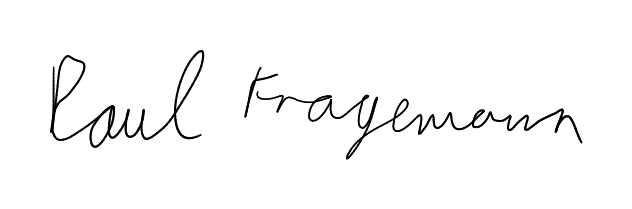
\includegraphics[width=5cm]{./assets/unterschrift}
\end{center}
\newpage

\section{Anhang}\label{sec:anhang}

\begin{figure}[h]
    \centering
    \input{visuazation_listing.txt}
    \caption{Minimax Visualisierung\protect\footnotemark }
    \label{fig:minimax-visulisation}
\end{figure}
\footnotetext{Eigenes Beispiel, Graphiken erstellt mit: \url{https://raphsilva.github.io/utilities/minimax_simulator/}}

    \label{code}
\label{piece_square_tables}

\end{document}